
% \section{提出优化函数}

\begin{frame}
  \frametitle{Poloidal Cross-section Analysis}
  \begin{figure}[t]
      \centering
      \subfloat[极向磁面磁场流图,图中还有一条 2D 磁力线紧贴着闭合磁面。]{%
        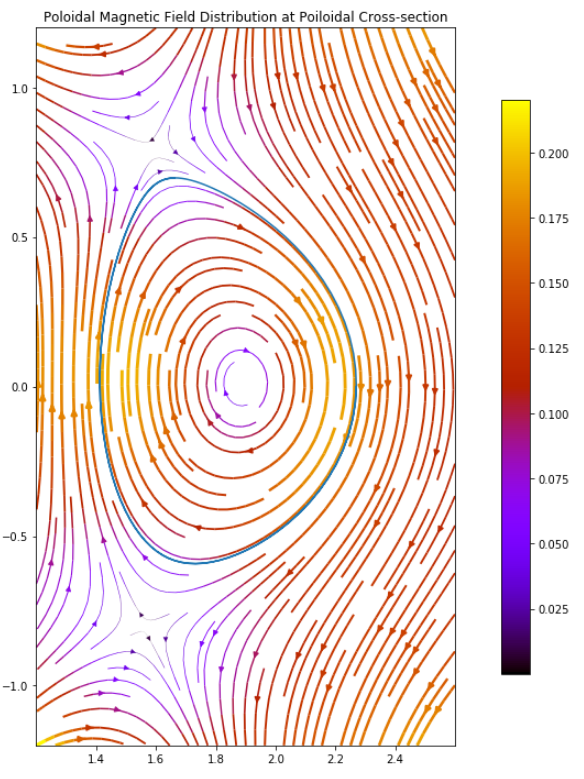
\includegraphics[width=0.45\columnwidth,keepaspectratio]{B_fiel_stream.png}
      }\hfill
      \subfloat[磁面坐标半径分布]{%
        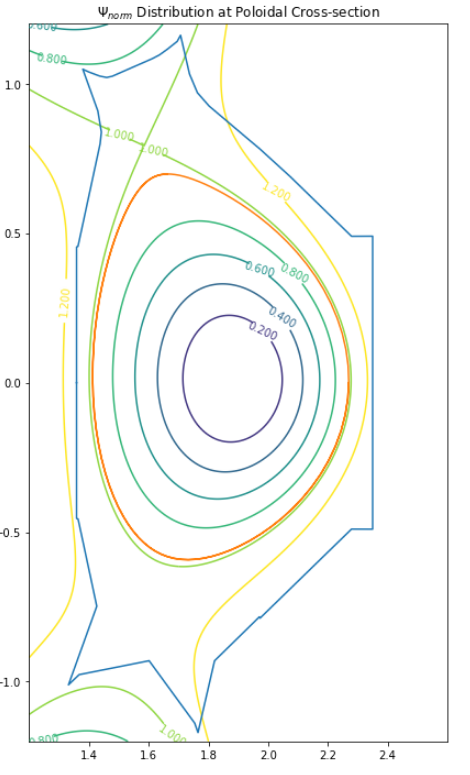
\includegraphics[width=0.37\columnwidth,keepaspectratio]{poloidal_B_surface}
      }%
  \end{figure}
\end{frame}



\begin{frame}
  \frametitle{Helical Current Filaments induced by LHW}
编写了螺旋电流丝沿磁力线运动的程序。
\begin{figure}[t]
  \centering
  \subfloat[\east 以氦气放电实验来用可见光显著地表现螺旋电流丝的三维几何分布,低杂波天线截图置于图中间。]{%
    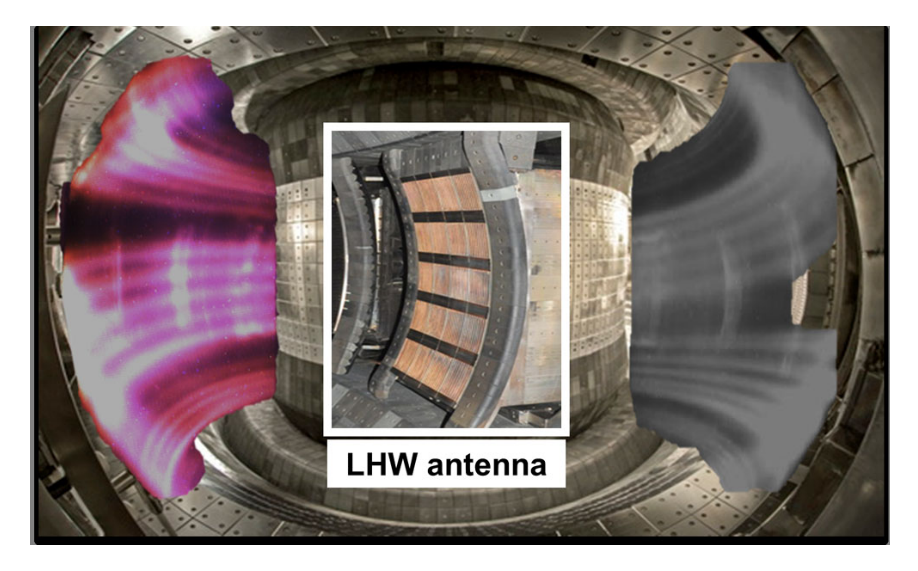
\includegraphics[width=0.35\columnwidth,keepaspectratio]{hcf/hcf_visible_image.png}
  }\hfill
  \subfloat[基于磁力线追踪计算得到的螺旋电流丝轨迹,五条分别螺旋电流丝起点分别取为五排低杂波天线的中间位置正对着的闭合磁面外 10 mm。]{%
    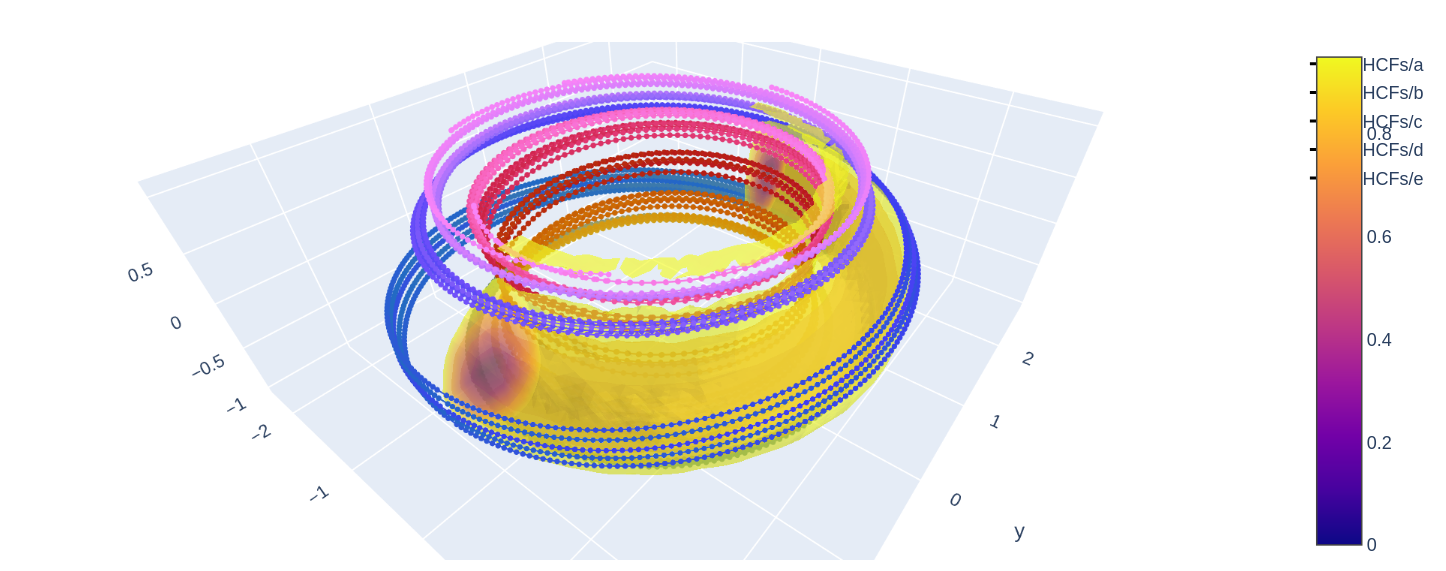
\includegraphics[width=0.6\columnwidth,keepaspectratio]{73999_030400ms_improved/hcfs_east.png}
  }%
\end{figure}
\end{frame}

\begin{frame}
  \frametitle{Helical Current Filaments induced by LHW}
编写了螺旋电流丝沿磁力线运动的程序,并将其保存为线圈一样的表格格式,但记录的是柱坐标。该程序另一方面在以后的第一壁载荷优化问题中可以再进行拓展。
\begin{figure}[htbp]
  \centering%
      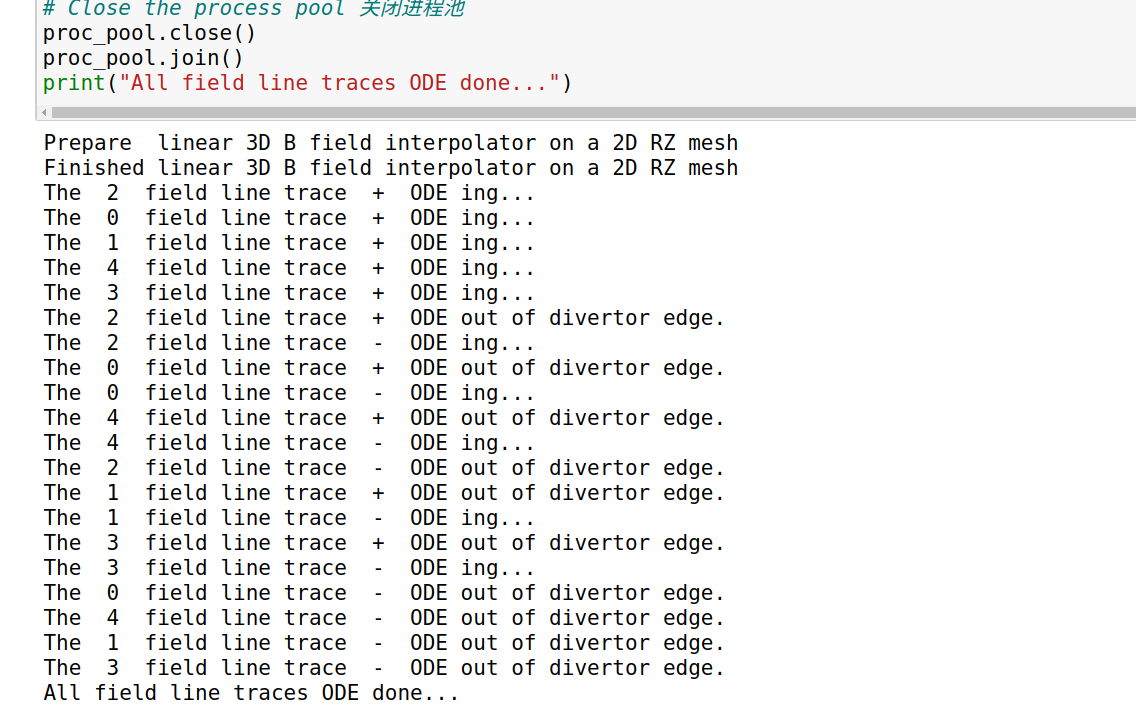
\includegraphics[width=0.8\columnwidth]{73999_030400ms_improved/flt_code_report.png}
      \caption{迹线追踪程序打到壁上会进行 out of divertor 的示意。}
\end{figure}
\end{frame}


\begin{frame}
  \frametitle{Perturbant Field Calculation }
  直接根据扰动场线圈 XYZ 点集工程数据并行计算场分量,改变了原有 ERGOS 需要对每个线圈进行磁场程序单独编写的工作,并且能够充分利用 CPU 。添加了方便的坐标变换函数,减少了日后其他科研人员需要产生磁场数据的工作量。

  \begin{figure}[htbp]
    \centering%
        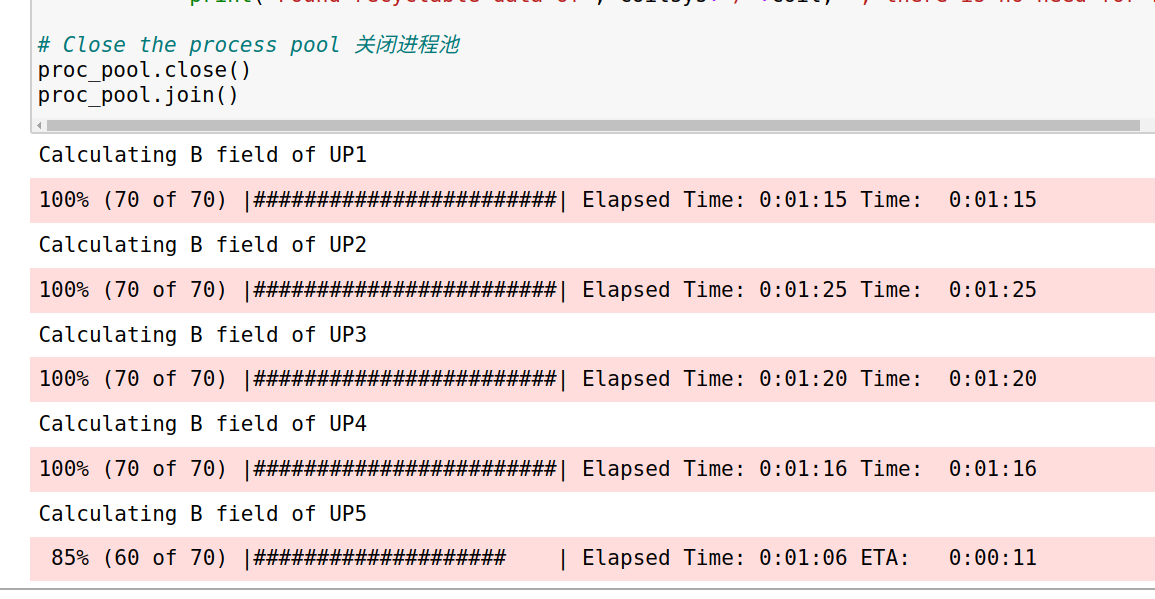
\includegraphics[width=0.8\columnwidth]{73999_030400ms_improved/B_field_calc_low_n.png}
        \caption{并行多核计算磁场分布的程序。}
  \end{figure}
\end{frame}

\begin{frame}
  \frametitle{Coil Collaboration}
  $$\tilde{b}_{m n}^{1}(s) \equiv \int_{\varphi=0}^{2 \pi} \int_{\theta^{*}=0}^{2 \pi} \tilde{b}^{1}\left(s, \theta^{*}, \varphi\right) e^{-i\left(m \theta^{*}+n \varphi\right)} \frac{d \theta^{*}}{2 \pi} \frac{d \varphi}{2 \pi}$$

  $$\tilde{b}^{1}\left(s, \theta^{*}, \varphi\right)=\sum_{m, n=-\infty}^{\infty} \tilde{b}_{m n}^{1}(s) e^{i\left(m \theta^{*}+n \varphi\right)}$$

  傅里叶变换的线性性、平移性大大减少了计算磁谱的成本。

  低 n 线圈电流强度的随着设置相位的变化利用线性性。
  高 m 线圈在 $\varphi$ 正方向上进行移动 $\Delta \varphi$,相当于$\tilde{b}_{m n}^{1}(s)$乘因子 $e^{-i\left(n \Delta\varphi \right )}$。

  在没有考虑电流强度不变的情况下,参数可选的空间相当于$\Phi_{UP}, \Phi_{DOWN}, \phi_{\text{high m}}$ $[0, 2\pi]\times[0,2\pi]\times[0,2\pi]$。

\end{frame}

\begin{frame}
  \frametitle{Coil Collaboration}
  近期将自己编写的磁场输入 ERGOS 进行磁谱计算的试验一方面发现,虽然磁场计算程序没写错,但还有些问题。

  \begin{enumerate}
    \item 磁场是从工程表格中从上到下设置为默认方向,设置电流符号相同时未检验在垂直磁面分量主要符号是否相同。当前进展还需加快,要早点发现这种小问题。
    \item 对于单边 Single-Null 的位型,上下两侧扰动场线圈产生的扰动场大小明显不同,使得电流相对大小参与到优化中更有必要了一些。
  \end{enumerate}

  
  \begin{figure}[htbp]
    \centering%
    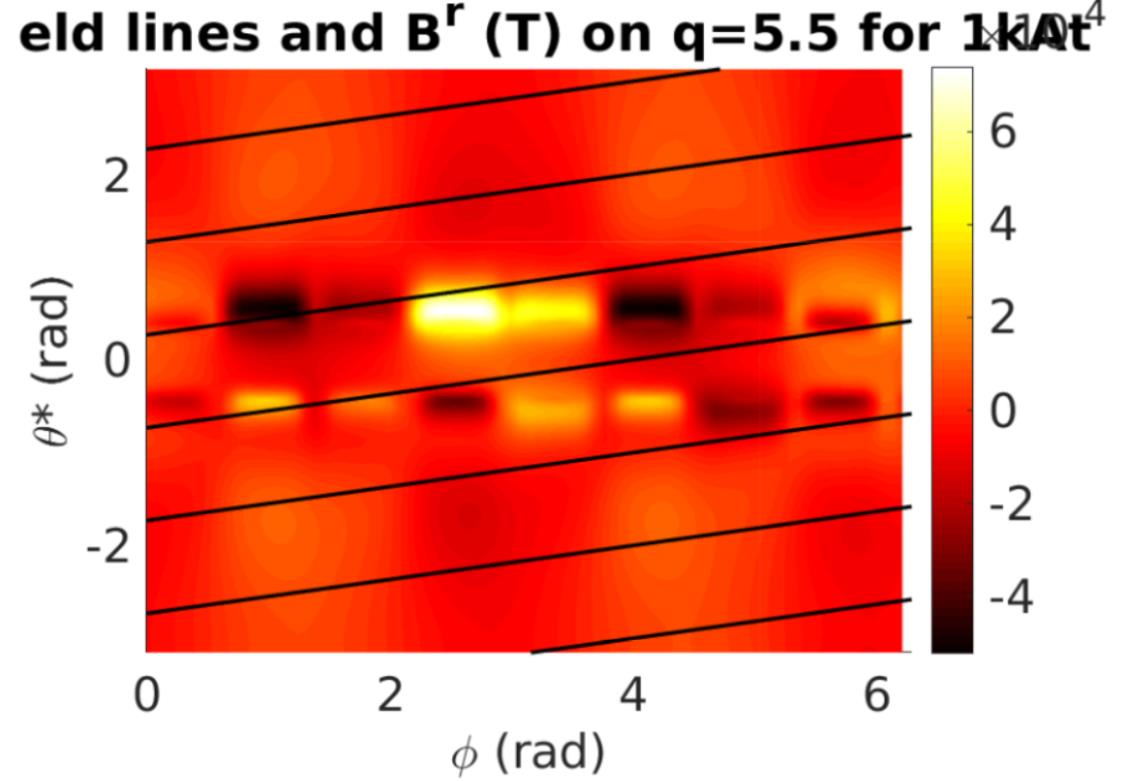
\includegraphics[width=0.45\columnwidth]{Br_flux_surface_q=5_5.jpg}
    \caption{RMP 低 n 线圈工作模式为 Even 时扰动场在 EAST\#73999 $q=5.5$ 磁面上的垂直磁面方向分量的分布。(by ERGOS\cite{nardon_edge_2007})}
  \end{figure}
  
\end{frame}


\begin{frame}
  \frametitle{Coil Collaboration}
  近期将自己编写的磁场输入 ERGOS 进行磁谱计算的试验一方面发现,前期工作还有些问题。从第一次最粗糙的计算来看磁谱 $\tilde{b}^1_{mn}$ 的迹线和各磁面安全因子对应的曲线贴合程度不足。
  

  \begin{figure}[t]
    \centering
    \subfloat[RMP 低 n 线圈工作模式为 Even 时扰动场在 EAST\#73999 $q=5.5$ 磁面上产生的磁谱 $\tilde{b}^1_{mn}$ 。(by ERGOS\cite{nardon_edge_2007})]{%
      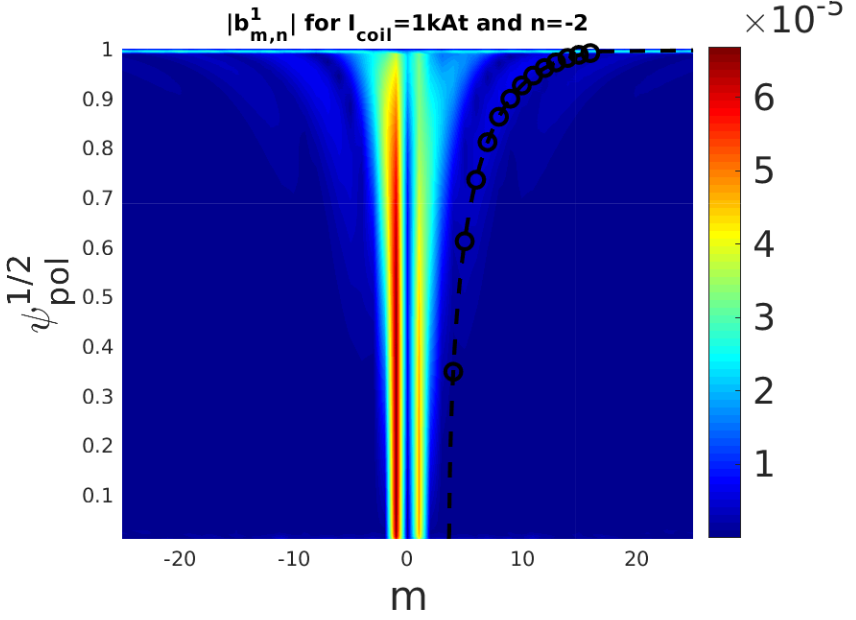
\includegraphics[width=0.35\columnwidth,keepaspectratio]{73999_030400ms_improved/spectrum_1kAt.png}
    }\hfill
    \subfloat[RMP 低 n 线圈各工作模式下下侧线圈电流分布,图中用光滑曲线拟合,实际为阶梯函数。Even 偶连接模式为上下侧线圈没有]{%
      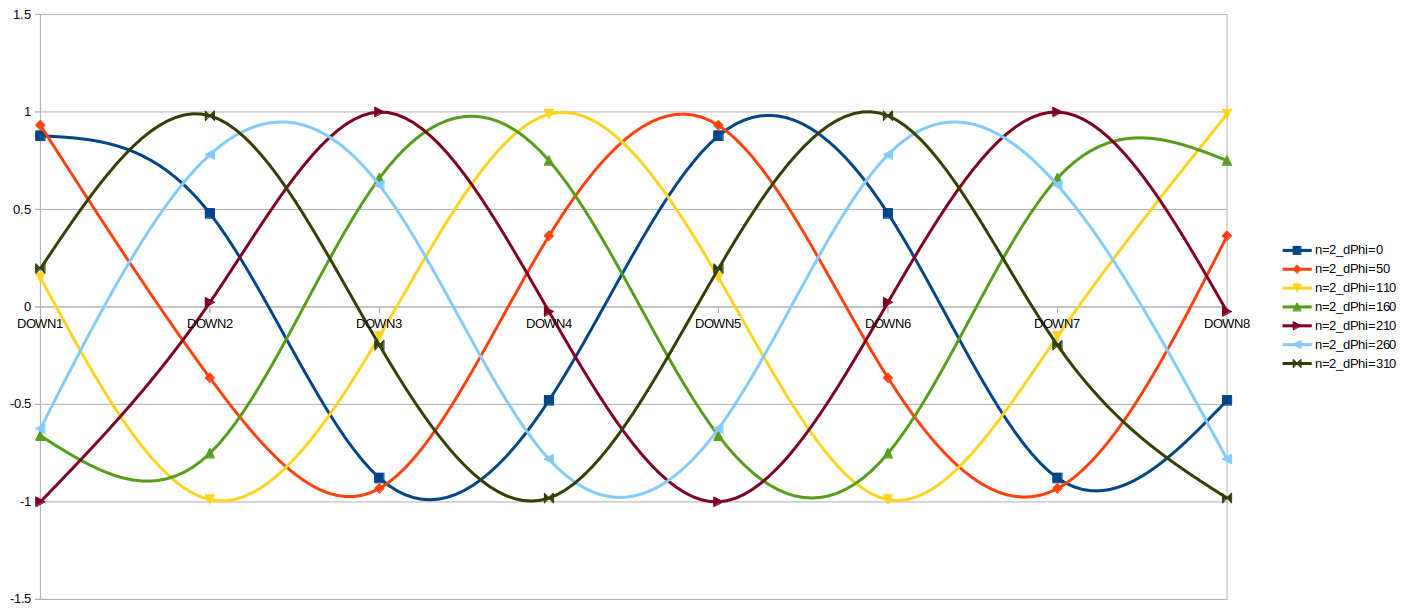
\includegraphics[width=0.6\columnwidth,keepaspectratio]{73999_030400ms_improved/low_n_coils_current.png}
    }%
  \end{figure}
  
\end{frame}




\begin{frame}
  \frametitle{Discussion}

  \begin{itemize}
    \item 程序接口问题,ERGOS Matlab 程序函数作者习惯没有输入输出,变量都是以 Matlab 内部变量储存。
    \item 对角度 $\varphi$ 这种有界参数,优化问题可以做一个扫描。但一旦引入了各扰动场的相对大小,优化方法可能就必需了。但 ERGOS 只适合串行,考虑将 ERGOS 中计算 Chirikov 径向分布计算等部分单独抽出来。FFT 可以不抽出来,因为线性性和平移性对每个线圈做一次计算就可以了。
  \end{itemize}
  
\end{frame}